%% LyX 2.0.1 created this file.  For more info, see http://www.lyx.org/.
%% Do not edit unless you really know what you are doing.
\documentclass[english]{article}
\usepackage[T1]{fontenc}
\usepackage{natbib}
\usepackage[applemac]{inputenc}
\usepackage[a4paper]{geometry}
\geometry{verbose,tmargin=2cm,bmargin=2cm,lmargin=2.5cm,rmargin=2.5cm}
\usepackage{float}
\usepackage{amsmath}
\usepackage{amsfonts}
\usepackage{graphicx}


\title{Adaptive and Discriminative Metric Differential Tracking}
\author{Gabriele Barni\\Tommaso Garuglieri}

\usepackage{subfig}

\begin{document}

\maketitle

\section*{Introduzione}

L' obiettivo di questa esercitazione \`e quello di sperimentare una tecnica di tracking in sequenze video, che incorpora una metrica adattiva all' interno del metodo di tracking differenziale. Questo tipo di approccio prevede una fase di learning  per l' addestramento di una metrica ottima derivata dalla metrica Mahalanobis,  e quindi il calcolo della stima del moto in forma chiusa.
\newline\newline
La scelta di una metrica  appropriata � fondamentale nelle performance delle operazioni di tracking, poich� ne determina la sua accuratezza e robustezza. A differenza di altre tecniche di tracking, il matching viene costruito direttamente tra due frame consecutivi, richiedendo cos� una soluzione computazionalmente pi� efficiente. Fondamentale, per le performance, � la scelta dello spazio delle feature : individuando uno spazio di feature forti (invarianti a cambi di luci e deformazioni locali) si riescono a ottenere buoni risultati anche utilizzando la semplice distanza Euclidea come metrica, ma laddove questo non � possibile, la scelta della metrica diventa fondamentale.
\newline\newline
A differenza degli altri metodi che utilizzano una metrica predefinita, il metodo qui studiato permette una migliore separabilit� del target dal background e da altri elementi di disturbo. Questo metodo non si limita soltanto alle feature legate al colore, ma � applicabile anche ad altre.

\section*{Pipeline del tracker}

La pipeline del tracker studiato prevede i seguenti passaggi : 
\begin{itemize}

\item Individuazione del target da tracciare, questo pu� essere eseguito specificando nel dettaglio le relative coordinate nel primo frame del video, oppure tramite una scelta manuale, sempre sul primo frame del video, della regione di interesse. Una volta individuato il target, se ne calcola l' istogramma nello spazio di feature scelto;

\item Fase di training per l' addestramento della metrica adattiva : questa � supervisionata, e consiste nell' individuazione di un insieme di esempi,  positivi e negativi : gli esempi positivi sono individuati nelle regioni del frame immediatamente vicine al target, mentre gli esempi negativi sono individuati in quelle regioni attorno al target. Per ogni esempio preso, se ne calcola l' istogramma, nello stesso spazio delle feature, e con la stessa tecnica, con cui � stato calcolato l' istogramma del target. Questa fase si conclude con l' individuazione della matrice $\mathbf{A} \ \mathcal{2} \ \mathbb{R}^{d \times m}$ (con $d \leq  m$), mediante la tecnica di Neighbourhood Components Analysis, descritta in \cite{main3},  che permette di ottenere un' alto livello di classificazione degli esempi di training.

%, massimizzando l' errore di classificazione  in the leave-one-out cross validation. This is achieved by adopting the soft-max formulation for the nearest-neighbor classification.
%
%come risultato di un processo di massimizzazione della funzione $g(\mathbf{A})$ (funzione che esegue una classificazione degli esempi di training) utilizzata poi nella metrica del tracker;

\item  Fase di tracking : per ogni frame, a partire dal target e da una regione candidata, viene calcolato lo spostamento ottimo, $\Delta c$ mediante l' utilizzo della matrice $\mathbf{A}$ : da esso viene quindi effettuata la predizione sulla posizione, nel frame successivo, del target. La fase di tracking prevede, inoltre, che per ogni frame vengano raccolti un insieme di esempi positivi e negativi, e, in base ad una soglia, il ricalcolo della matrice $\mathbf{A}$.

\end{itemize}

\section*{Strumenti utilizzati}

Per l' implementazione, e quindi la successiva fase di sperimentazione, dell' algoritmo, si utilizza Matlab.\\\\
La fase di addestramento della metrica viene eseguito mediante il toolbox, scritto in Matlab, messo a disposizione dagli autori di \cite{main3}, che a partire dall' insieme di campioni positivi e negativi, opportunamente etichettati, permette di ottenere la matrice di trasformazione $\mathbf{A}$. In particolare, il problema di massimizzazione viene convertito in uno di minimizzazione, e viene  quindi richiamata la funzione di minimizzazione che permette quindi di ottenere la matrice che rende massima la classificazione.


\section*{Adaptive Metric Learning}

Seguendo i passaggi in \cite{main1}, si considera la distanza di Mahalanobis : 

$$ \mathcal{D}(\mathbf{x}_{i},\mathbf{x}_{j} ) = (\mathbf{Ax}_i -  \mathbf{Ax}_j )^T (\mathbf{Ax}_i -  \mathbf{Ax}_j ) 
= (\mathbf{x}_i -  \mathbf{x}_j )^T \mathbf{Q}(\mathbf{x}_i -  \mathbf{x}_j ) $$

Questa viene parametrizzata mediante l' uso della matrice $\mathbf{A} \ \mathcal{2} \ \mathbb{R}^{d \times m}$, che, mediante una trasformazione lineare, trasforma  lo spazio originario delle feature, $\mathbb{R}^m$, in un nuovo spazio $\mathbb{R}^d$ (dove $d \leq m$). La matrice $\mathbf{Q} = \mathbf{A}^T\mathbf{A}$. 
%Una volta acquisiti i dati di training (campioni positivi e campioni negativi) otteniamo quindi la matrice $\mathbf{A}$. 
Questa permette di riportarci in un nuovo spazio, dove la distanza fra i dati di una stessa classe viene ridotta, mentre viene aumentata quella rispetto ad i dati di una classe differente. 

\begin{figure}[ht]
\centering
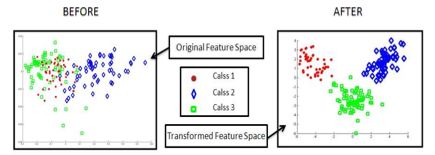
\includegraphics[scale=0.6]{screen2.png}
\caption{Esempio di trasformazione dei dati tramite la matrice $\mathbf{A}$}
\end{figure}
\vspace{0.3cm}

Come precedente introdotto, la fase di learning prevede l' acquisizione di un set di campioni positivi e un set di campioni negativi. A partire dalla regione di interesse (target) i campioni positivi vengono acquisiti in quelle regioni ottenute spostando la regione del target di pochi pixel. I campioni negativi, invece, vengono individuati in quelle regioni che possono creare problemi di falsi positivi.

\begin{figure}[ht]
\centering
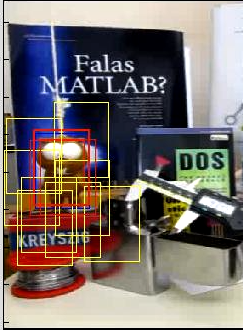
\includegraphics[scale=0.5]{screen1.png}
\caption{Esempio di acquisizione di campioni positivi,in rosso, e negativi, in giallo}
\end{figure}

%%mettere immagine di esempio
\vspace{0.3cm}
In base ai dati acquisiti, il tracker � in grado di eseguire una classificazione accurata, oltre a non avere problemi legati all' individuazione di falsi positivi. La matrice $\mathbf{A}$  permette di ottenere le migliori performance di classificazione, per un classificatore di tipo Nearest Neighbour (k-NN), nel nuovo spazio a $d$ dimensioni. Il classificatore esegue una predizione sulla classe di un dato in ingresso in basse alle informazioni sui k dati pi� vicini, in base a una metrica data. Questo metodo non � comunque differenziabile rispetto ad $\mathbf{A}$, per questo viene utilizzata una rappresentazione pi� semplice dei nearest neighbours. Dato l' insieme di vettori del training set $x_1, x_2, ... , x_n \ \mathcal{2} \ \mathbb{R}^m$, con le corrispondenti etichette  delle relative classi $c_1,c_2, ... , c_n$, si misura la relazione di vicinanza tra due coppie di vettori $x_i$ e $x_j$ mediante una misura probabilistica $p_{ij}$ : 
$$p_{ij} = \frac{\text{exp}(-\| \mathbf{A}x_i - \mathbf{A}x_j  \| ^2)}{ \sum_{k \neq i} \text{exp}(-\| \mathbf{A}x_i - \mathbf{A}x_k  \| ^2)}.$$

Quindi ogni vettore di feature $x_i$,  tratta un altro vettore $x_j$ con probabilit� $p_{ij}$, e ereditandone l' etichetta relativa alla classe. Possiamo quindi individuare la probabilit� $p_i$ che il punto $i$ venga correttamente classificato :

$$p_i=\sum_{j \mathcal{2} C_i} p_{ij}$$

dove $C_i = \{ j | c_i = c_j \}$. L' obiettivo � quindi quello di massimizzare il numero di punti del training set correttamente classificati. Per far ci� viene utilizzata la seguente funzione obiettivo : 

$$ g(\mathbf{A}) = \sum_i log( \sum_{j \mathcal{2} C_i} p_{ij}) = \sum_i log(p_i) .$$

Quindi l' obiettivo � quello di individuare la trasformazione $\mathbf{A}$ che massimizzi il numero di punti correttamente classificati nel training set, cio� :

$$\mathbf{A^*} = \arg \max_{\mathbf{A}} g(\mathbf{A}).$$

Questo problema di ottimizzazione pu� essere affrontato mediante una qualsiasi tecnica basata sul gradiente, dato che quello della funzione $ g(\mathbf{A})$ pu� essere ottenuto in forma chiusa :

$$ \frac{\partial g}{\partial \mathbf{A}}  = 2\mathbf{A} \sum_i (\sum_k  p_{ik} x_{ik} x_{ik}^T - \frac{\sum_{j \mathcal{2} C_i} p_{ij}x_{ij}x_{ij}^T}{\sum_{j \mathcal{2} C_i} p_{ij}})$$

dove $x_{ij} = x_i - x_j$.

%%da chiarire ? e concludere

\section*{Adaptive Metric Differential Tracking}

La tecnica di tracking utilizzata, differential tracking, assume che tra un frame e l' altro vi siano piccoli spostamenti del target.
Come tutti i metodi di tracking basati sull' uso di una funzione kernel, questo prevede che l' istogramma della regione del target che si vuol tracciare, venga pesato spazialmente mediante l' uso di una funzione kernel. Come descritto in \cite{main2}, sia $\{\mathbf{x}_i\}_{i=1...n}$ l' insieme dei pixel della regione del target nel frame della sequenza video. Dati $\mathit{F}$, lo spazio delle feature utilizzato, e  $\mathit{U} = 1 ... m$, un numero finito di "bins", sia $b = \mathit{F} \to \mathit{U}$ una funzione di "binning" : $b(\mathbf{x},t)$ indica il bin corrispondente alla feature del pixel $\mathbf{x}$, al tempo $t$. Sia, infine, $\mathbf{K}: \Re^2 \to \Re^+ $, la funzione kernel che "pesa" i pixel della regione del target. Quindi, l' istogramma delle feature della regione del target $\mathbf{q} = [q_1, q_2, ... , q_m] ^ T \ \mathcal{2} \ \mathbb{R}^m$, viene calcolato come: 

$$q_u \ = \ C\sum_{i=1}^n{K}(\mathbf{x}_i - \mathbf{c})\delta(b(\mathbf{x}_i,t),u)$$
$$C\ = \ \frac{1}{\sum_{i=1}^n{K}(\mathbf{x}_i - \mathbf{c})}$$

dove $\delta$ � il delta di Kronecker, mentre $\mathbf{c}$ � il centro del kernel. Notiamo che, per come viene definito $C$, si avr� che $\sum_{u=1}^m q_u = 1$. Il calcolo di $\mathbf{q} $ pu� essere riscritto con una formulazione pi� compatta, mediante una formulazione matriciale :

$$\mathbf{q(c)} = \mathbf{U}^T \mathbf{K(c)} $$

dove $\mathbf{U} $, matrice dei bin, � : 

$$\mathbf{U} = \begin{bmatrix} \delta(b(y_1),u_1) & \cdots & \delta(b(y_1),u_m) \\  \vdots & \ddots & \vdots \\ \delta(b(y_n),u_1) & \cdots & \delta(b(y_n),u_m)  \end{bmatrix}  \mathcal{2} \ \mathbb{R}^{n \times m}$$

mentre,  $\mathbf{K} $, la matrice del kernel : 

$$\mathbf{K(c)} = \begin{bmatrix} K(y_1 - c) \\ \vdots \\ K(y_n - c) \end{bmatrix}  \mathcal{2} \ \mathbb{R}^{n}.$$

Indichiamo con $\mathbf{p(c+ \Delta c)}$ l' istogramma del target candidato, e con $D(\mathbf{q(c), p(c+ \Delta c)})$ la funzione obiettivo nella fase di matching, l' obiettivo del tracker � quello di individuare il miglior discostamento $\Delta c$, tale da minimizzare la funzione obiettivo : 

$$\mathbf{ \Delta c ^* } = \arg \min_{\mathbf{ \Delta c}} D(\mathbf{q(c), p(c+ \Delta c)})  $$

Il discostamento ottimale viene ottenuto come :

$$\mathbf{ \Delta c ^*  = (M^T A^T A M)^{-1}  M^T A^T A (\sqrt{q} - \sqrt{p(c)}) },$$

dove $\mathbf{ \Delta c} \ \mathcal{2} \ \mathbb{R}^{r}$, e 

$$\mathbf{ M = \frac{1}{2} \text{diag}(p(c))^{(-\frac{1}{2})} \mathbf{ U^T J_K(c)} } \ \mathcal{2} \ \mathbb{R}^{m \times r},$$

$$\mathbf{J_K} = \begin{bmatrix} \mathcal{5}_c K(y_1 - c) \\ \vdots \\ \mathcal{5}_c K(y_n - c) \end{bmatrix}  \mathcal{2} \ \mathbb{R}^{n \times r}.$$

%\section*{Implementazione}


\section*{Sperimentazione}

In tutti gli esperimenti viene effettuata la selezione dei campioni positivi e negativi viene effettuata mediante l' utilizzo di un generatore di numeri pseudocasuali, distribuiti secondo una distribuzione normale, come si pu� vedere in \figurename~\ref{screen3}.

\begin{figure}[ht]
\centering
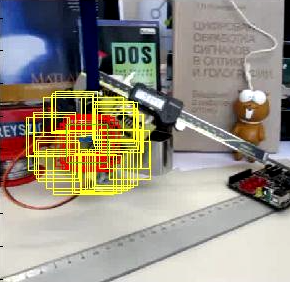
\includegraphics[scale=0.6]{screen3.png}
\caption{Esempio di acquisizione dei campioni secondo una distribuzione normale, durante la fase di training. In giallo i campioni negativi, mentre in rosso quelli positivi, in verde il target.}
\label{screen3}
\end{figure}
\vspace{0.3cm}

Inoltre, nella fase di tracking, vengono acquisiti nuovi campioni positivi e negativi, e, insieme ad i campioni pi� recenti, acquisiti durante la fase di training, viene calcolato il valore della funzione $g(\mathbf{A})$. Se il valore della funzione oltrepassa una soglia predefinita, viene effettuato un nuovo addestramento della metrica, ottenendo quindi una nuova matrice $\mathbf{A}$.

Per quanto riguarda l' addestramento della metrica, la funzione che si occupa della massimizzazione della funzione $g(\mathbf{A})$, prevede che vengano impostate un numero di iterazioni dell' algoritmo. Per ogni iterazione viene restituito un valore della funzione e la corrispondente matrice $\mathbf{A}$. Nell' implementazione del tracker non viene impostato un numero fissato di iterazioni, ma mediante un valore predefinito di una soglia, viene ripetuto il processo di massimizzazione fino al raggiungimento di un determinato valore della funzione.\\\\

Gli esperimenti effettuati si distinguono quindi per i seguenti fattori :
\begin{itemize}
\item modalit� di scelta dei campioni;
\item numero di campioni positivi e negativi scelti;
\item soglia sul valore di $g(\mathbf{A})$ per il ricalcolo della matrice $\mathbf{A}$;
\item soglia sul valore di $g(\mathbf{A})$ nel processo di addestramento della metrica;
\item spazio delle feature.
\end{itemize} 

Sperimentazioni effettuate sui video di test e relativi commenti. Elenco quindi dei video dove la tecnica produce buoni risultati ma anche di video dove la tecnica incontra difficolt� nel tracking. descrizioni nell' impostazione dei parametri utilizzati : numero di campioni positivi e negativi utilizzati per l' addestramento , e ad ogni frame, sogli per le intersezioni nella selezione dei campioni positivi e negativi, soglia per il riaddestramento della metrica.

\section*{Conclusioni}

\newpage
\bibliographystyle{plain}
\bibliography{BIBLIO}
\end{document}

